\subsection{\large{\textit{cP}1-Po (Inverse)}}\vspace{-0.1in}
Inverse Simple Cubic


\begin{figure}[H]
\begin{minipage}{0.34\textwidth}\centering
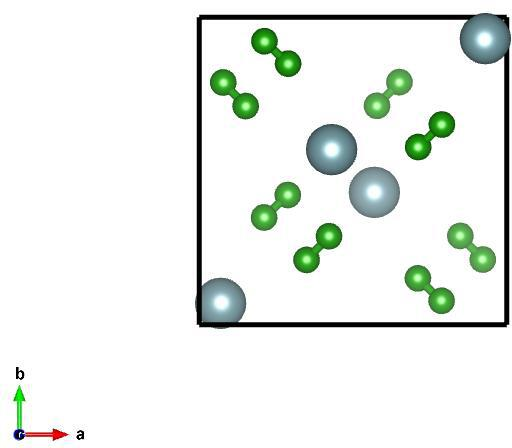
\includegraphics[width=0.9\linewidth,height=2in,keepaspectratio]{/Users/rosecers/work_folders/structures_for_photonics/reference/ref_inp/workspace/d3e0b4d3ebe976416944b0f4fdec40b4/final_images/analog_trim.jpg}\\
\small{Image of \textit{cP}1-Po, generated by Vesta}
\end{minipage}\hfill
\begin{minipage}{0.65\textwidth}\raggedright
{\setlength{\mathindent}{0cm}
\begin{equation*}
\begin{split}&\boldsymbol{a_1} = \ \hat{x}\\[-8pt]
&\boldsymbol{a_2} = \ \hat{y}\\[-8pt]
&\boldsymbol{a_3} = \ \hat{z}
\end{split}
\end{equation*}}

\textbf{Space Group:}	221\hspace{0.5in}\textbf{Point Group:}	$m\bar{3}m$\\
\textbf{Inorganic Crystallographic Database} \#43211\\
\textbf{Structure DOI: }\url{10.1016/0022-1902(66)80270-1}

\end{minipage}\hfill
\end{figure}
\vspace{-0.25in}


\begin{figure}[H]
\begin{minipage}{0.9\textwidth}\centering
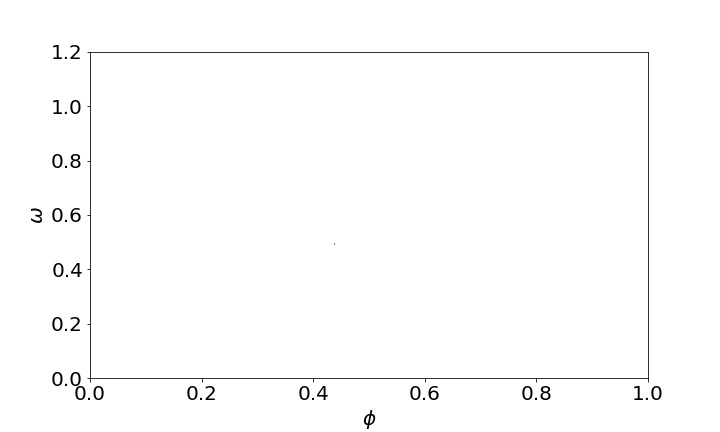
\includegraphics[width=0.9\linewidth,height=2.5in,keepaspectratio]{/Users/rosecers/work_folders/structures_for_photonics/reference/ref_inp/workspace/d3e0b4d3ebe976416944b0f4fdec40b4/final_images/gap_atlas.jpg}
\\
\end{minipage}\hfill\caption{Gap Atlas across filling fraction $\phi$ and frequency $\omega$}
\end{figure}


\begin{figure}[H]
\begin{minipage}{0.5\textwidth}\centering
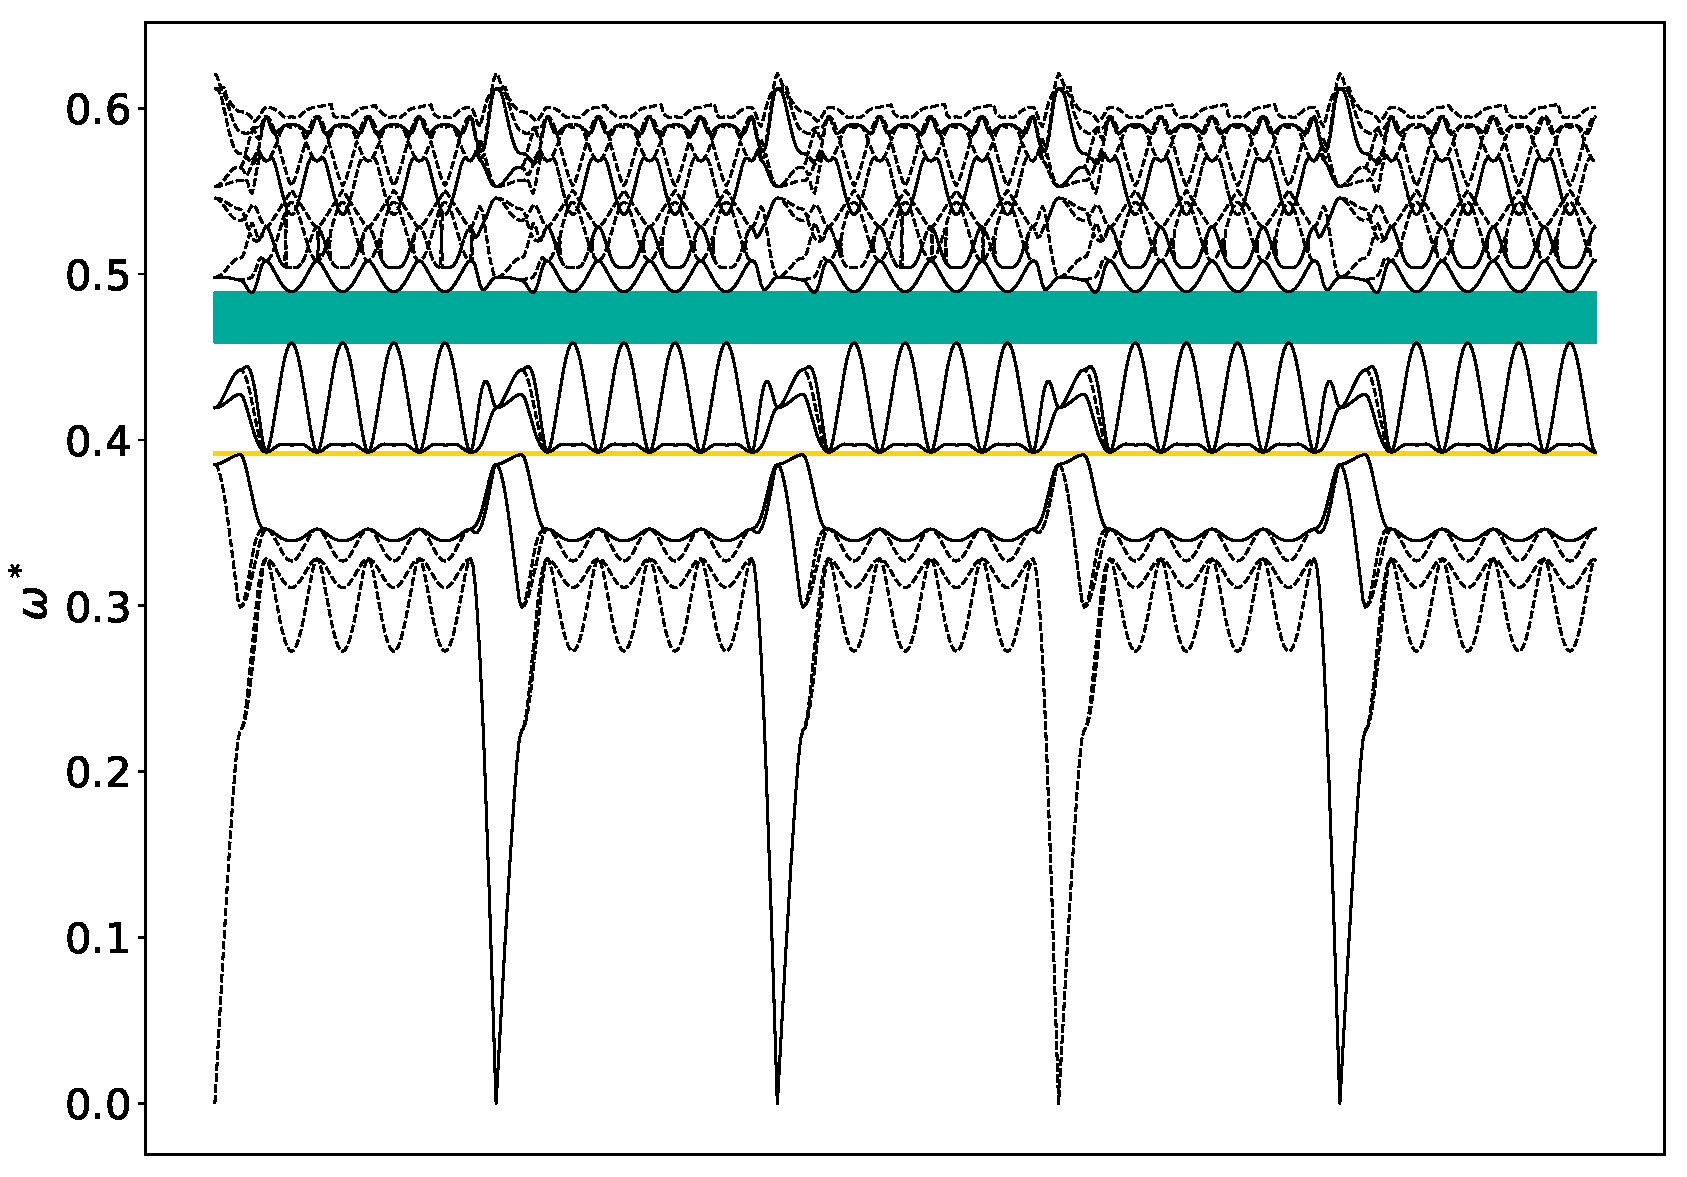
\includegraphics[width=0.9\linewidth,height=1.5in,keepaspectratio]{/Users/rosecers/work_folders/structures_for_photonics/reference/ref_inp/workspace/d3e0b4d3ebe976416944b0f4fdec40b4/./final_images/band_diagram_b=5.pdf}
\\Band Structure across 1st BZ
\end{minipage}\hfill
\begin{minipage}{0.48\textwidth}\centering
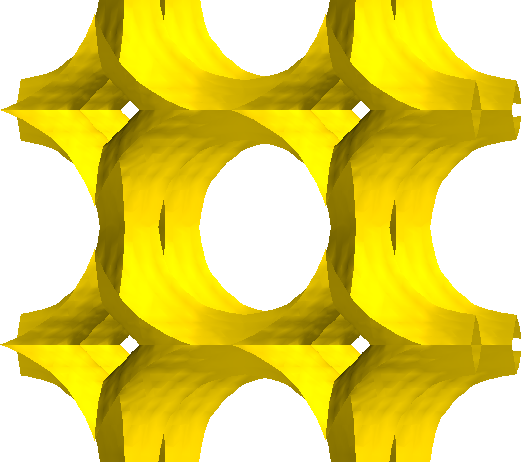
\includegraphics[width=0.9\linewidth,height=1.5in,keepaspectratio]{/Users/rosecers/work_folders/structures_for_photonics/reference/ref_inp/workspace/d3e0b4d3ebe976416944b0f4fdec40b4/final_images/cP1-Po_r@gap_5-6.png}
\\View along $a_3$ 
\end{minipage}\hfill\caption{Band Structure and Isosurface of \textit{cP}1-Po (Inverse) at radius = 0.61, filling fraction = 0.18, where the largest gap between bands 5 and 6 occurs with gap size 11.58\%.}

\end{figure}
\vspace{-0.25in}

